% Layout-only illustration owned by report; not an experimental figure.
\begin{figure}[pos=H]
\centering
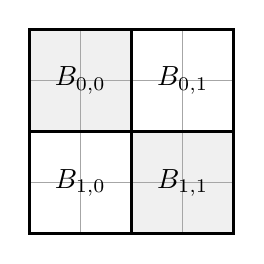
\begin{tikzpicture}[scale=0.65]
  \fill[gray!12] (0,2) rectangle (2,4);
  \fill[gray!12] (2,0) rectangle (4,2);
  \draw[step=1,gray!70,thin] (0,0) grid (4,4);
  \draw[line width=1.1pt] (0,0) rectangle (4,4);
  \draw[line width=1.1pt] (2,0)--(2,4) (0,2)--(4,2);
  \node at (1,3) {$B_{0,0}$};
  \node at (3,3) {$B_{0,1}$};
  \node at (1,1) {$B_{1,0}$};
  \node at (3,1) {$B_{1,1}$};
\end{tikzpicture}
\caption{\lang{Sơ đồ bốn khối của bảng $4\times4$ với $n=2$.}{Block layout of a $4\times4$ grid with $n=2$.}}
\label{fig:blocks}
\end{figure}
